\chapter{Vector Autoregressive Models}

\section{VAR Analysis}

A Vector Autoregressive model of order $p$, denoted as $\text{VAR}(p)$, is used to model multivariate time series where each variable depends linearly on its own past values and those of other variables in the system. In contrast to univariate autoregressive models, VAR models account for the interdependencies among multiple time series by allowing each variable in the system to depend not only on its own past values but also on the past values of all other variables. This makes VAR particularly suitable for analyzing financial and economic systems where variables are often jointly determined, such as stock returns.

For $k-$dimensional time series $r_t$, the $\text{VAR}(p)$ model is specified as 
\begin{equation}
	r_t=\phi_0+\Phi_1 r_{t-1}+\cdots+\Phi_pr_{t-p}+a_t
\end{equation}
where $\Phi_0$ is a $k\times 1$ vector of constants, $\Phi_j$ is a $k\times k$ autoregressive coefficient matrix, and $a_t$ is a white noise innovation vector $\amsbb{E}[a_t]=0$ and $\text{Cov}(a_t)=\Sigma_a,$ a positive definite matrix.

One of the key strengths of VAR models is their ability to facilitate impulse response analysis, which tracks how a shock to one variable affects the entire system over time. This is useful in understanding transmission mechanisms, such as how a central bank interest rate change impacts inflation and output. Another common application is forecast error variance decomposition, which quantifies the contribution of each variable’s shock to the forecast error variance of others, offering insights into relative importance.

\begin{figure}[!h]
	\centering
	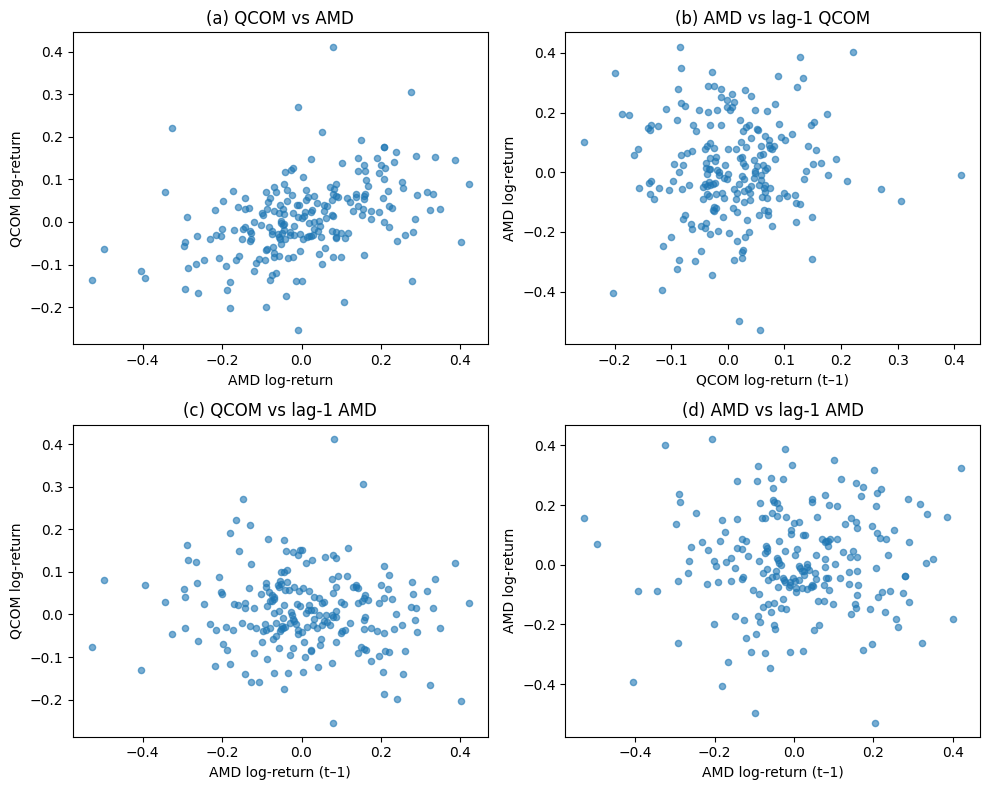
\includegraphics[width=0.8\linewidth]{content/plots/amd_qcom_scatter.png}
	\caption{Scatter Plot of Monthly log returns of AMD and QCOM}
	\label{fig:amd_qcom_scatter}
\end{figure}

Figure (\ref{fig:amd_qcom_scatter}) shows a panel of scatterplots, which illustrates the joint behavior and possible dynamic interactions between the monthly log returns of AMD and QCOM. In plot (a), which compares the concurrent log returns of QCOM and AMD, we observe a moderate positive association. This indicates that when AMD experiences a positive or negative return in a given month, QCOM tends to move in the same direction. This contemporaneous correlation suggests shared exposure to common market factors or industry-specific dynamics (both being semiconductor firms).

Plot (b) investigates whether QCOM’s past return (lag-1) helps explain AMD’s current return. The scatter shows weak structure and appears diffuse, suggesting limited predictive power from QCOM’s previous month return on AMD's current return. Likewise, plot (c) compares QCOM’s current return to AMD’s lag-1 return, and again, no strong relationship emerges, indicating that AMD’s past performance does not substantially inform QCOM’s present movement.

Finally, plot (d) looks at AMD's return against its own lag-1 value. The spread suggests minimal autocorrelation, which aligns with the empirical observation that individual stock returns are typically weakly autocorrelated at monthly frequencies due to market efficiency.

In our research, we we estimate a VAR(1) model using monthly log returns from QCOM (Qualcomm) and AMD (Advanced Micro Devices). The VAR(1) specification implies that each variable in the system is modeled as a linear function of one lag of both itself and the other variable, plus a constant and a random error term. This structure allows us to explore how past performance in one stock may influence future returns in both, offering insights into potential lead-lag relationships and co-movement dynamics in financial markets.

Matheamatically, a VAR(1) model for two variables can be expressed as the following:
\begin{equation}
	r_t=\phi_0+\Phi_{r_{t-1}}+a_t
\end{equation}

where $\phi_0$ is a $k-$dimensional vector, $\Phi$ is a $k\times k$ matrix, and $\lbrace a_t\rbrace$ is a sequence of serially uncorrelated random vectors with mean zero and covariance matrix $\Sigma$. The VAR(1) model consist of the following two equations:

\begin{equation}
	\begin{aligned}
		r_{1t}=\phi_{10}+\Phi_{11}r_{1,t-1}+\Phi_{12}r_{2,t-1}+a_{1t},\\
		r_{2t}=\phi_{20}+\Phi_{21}r_{1,t-1}+\Phi_{22}r_{2,t-1}+a_{2t},\\
	\end{aligned}
\end{equation}
The individual equations derived from the matrix form are QCOM returns:
\begin{equation}
	\begin{aligned}
		\text{QCOM}_t=0.002356\cdot\text{QCOM}_{t-1}+0.03490\cdot\text{AMD}_{t-1}+2.1352\\
		\text{AMD}_t=-0.03611\cdot\text{QCOM}_{t-1}-0.08491\cdot\text{AMD}_{t-1}+1.9618\\
	\end{aligned}
\end{equation}
which gives us the following matrix representation
\begin{equation}
	\begin{bmatrix}
		\text{QCOM}_t \\
		\text{AMD}_t
	\end{bmatrix}
	=
	\begin{bmatrix}
		2.1352 \\
		1.9618
	\end{bmatrix}
	+
	\begin{bmatrix}
		0.02356 & 0.03490 \\
		-0.03611 & -0.08491
	\end{bmatrix}
	\begin{bmatrix}
		\text{QCOM}_{t-1} \\
		\text{AMD}_{t-1}
	\end{bmatrix}
	+
	\begin{bmatrix}
		\epsilon_{\text{QCOM},t} \\
		\epsilon_{\text{AMD},t}
	\end{bmatrix}
\end{equation}
The QCOM equation shows weak positive autocorrelation and a mild positive effect from AMD’s previous return, suggesting slight predictive influence. The AMD equation exhibits negative coefficients for both lagged variables, indicating possible mean-reversion and a modest inverse relationship with QCOM’s past performance. The intercept terms represent average return levels adjusted for lagged influences.

Overall, the VAR(1) model captures the dynamic feedback between AMD and QCOM returns, allowing for richer modeling than univariate time series approaches. The small magnitude of the coefficients suggests that while interdependence exists, the direct predictive power is limited. However, even weak relationships can be valuable for short-term forecasting, constructing hedging strategies, or understanding market behavior under shocks (e.g., via impulse response functions). 

\section{Cointegration}

In financial time series analysis, it is common to observe that individual asset prices or economic indicators follow nonstationary behavior, typically modeled as integrated processes of order one, \( I(1) \). However, economic theory often suggests that certain groups of such variables move together in the long run, maintaining stable equilibrium relationships despite short-term fluctuations. This phenomenon is known as \textit{cointegration}. Formally, if \( x_{1t} \) and \( x_{2t} \) are both \( I(1) \) series, they are cointegrated if there exists a scalar \( \gamma \) such that the linear combination \( w_t = x_{1t} - \gamma x_{2t} \) is stationary (\( I(0) \)). The vector \( (1, -\gamma) \) is then called the cointegrating vector, and \( w_t \) represents the equilibrium error or spread.

To formally test and model cointegrated systems, particularly in higher dimensions, the \textit{Vector Error Correction Model (VECM)} framework is employed. This begins by rewriting a VAR(\(p\)) model of nonstationary series \( X_t \) in terms of first differences, yielding the VECM:
\begin{equation}
	\Delta X_t = \Pi X_{t-1} + \sum_{i=1}^{p-1} \Phi_i^* \Delta X_{t-i} + a_t
\end{equation}
Here, the matrix \( \Pi = \Phi_1 + \cdots + \Phi_p - I \) captures the long-run relationships, while \( \Phi_i^* \) represent short-run dynamics. The key insight is that the rank of \( \Pi \) determines the cointegration structure: if \( \text{rank}(\Pi) = r < k \), then there exist \( r \) cointegrating vectors, and we can factor \( \Pi \) as \( \alpha \beta' \), where \( \beta \) contains the cointegrating vectors and \( \alpha \) reflects the speed of adjustment toward long-run equilibrium.

\begin{figure}[!h]
	\centering
	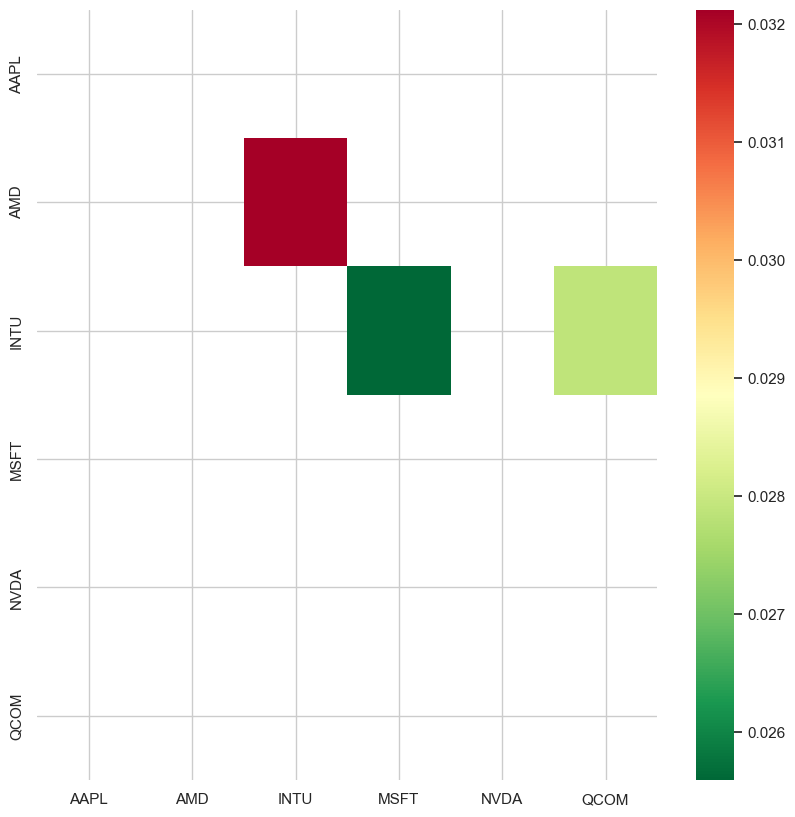
\includegraphics[width=0.5\linewidth]{content/plots/engle_granger.png}
	\caption{Cointegration Plot of Our Sample Securities using the Johansen Test}
	\label{fig:engle_granger}
\end{figure}

Cointegration has significant implications in financial applications. For instance, in pairs trading, if two stock prices are cointegrated, the spread \( w_t = p_{1t} - \gamma p_{2t} \) will be mean-reverting, allowing traders to exploit deviations from the equilibrium for profit. A trading strategy might involve taking a long position in one stock and a short position in the other when the spread deviates from its historical mean by a certain threshold. 

The Johansen test, based on estimating the rank of \( \Pi \) in the VECM, is the standard method for identifying such cointegrating relationships in multivariate systems. The hypothesis test is as follows:
\begin{equation}
	\begin{aligned}
		&H_0:\text{rank}(\Pi)\leq r\\
		&H_a:\text{rank}(\Pi)>r
	\end{aligned}
\end{equation}
So increasing the assumed rank and testing how many stationary combinations exists. 


Figure (\ref{fig:sample_securities}) shows the cumulative returns for securities in our universe. These securities are in the same industry as QCOM This involves assets such as AAPL, AMD, INTU, MSFT, NDVA, and QCOM. As we can see, some assets appear to move together, such as INTU, QCOM, MSFT, and AMD. Compared to AAPL and NVDA, they all have smaller cumulative returns. The question is whether these securites are cointegrated with QCOM. Figure (\ref{fig:engle_granger}) plots the heatmap of the Johansen test of the sample securites in our universe. The interval for the test is between 2017 and 2025. At the heat map shows, there are only three pairs of securities where we reject the null hypothesis of no cointegration: AMD with INTU, MSFT with INTU, and QCOM with INTU.

